\newif\ifPAPER  
\PAPERtrue % select either slide or note
%\PAPERfalse  

\def\g4{{\sf Geant4}}

\newcommand{\codeAlgorithm}[1]{
\addcontentsline{toc}{section}{Résumé}
\begin{center}\fbox{\parbox{12cm}{\bf #1}}\end{center}}

\newcommand{\cppintro}[1]{
\lstset{language=C,
caption= #1 ,
label=listing:boundary}}

\def\cppstart{\begin{lstlisting}}
\def\cppend{\end{lstlisting}}

\newif\ifCITENOTE 
\CITENOTEtrue

\ifPAPER
\documentclass[twoside,floatfix,a4wide]{d}
\usepackage{multirow}
\usepackage{url}
\usepackage{listings}
\usepackage{graphicx}
\usepackage{wrapfig}
%\usepackage{makeidx}
\usepackage{subfig}
\usepackage{fancyhdr}
%\usepackage{asymptote}
\usepackage{amsmath}
\usepackage{verbatim} % for comment
\usepackage{eurosym} 
\usepackage{color} % for definecolor
\usepackage[colorlinks,bookmarks=true]{hyperref}

\numberwithin{equation}{section} % reguires amsmath-package
\pagestyle{fancy}
\fancyhead{} % clear all fields

\fancyhead[L]{\it {Helsinki, May 4, 2009}} % Left Odd, Right Even 
\fancyfoot[L]{G.Danielsen - Simulating carbon beam fragmentation on water phantom with the Geant4 INCL/ABLA models} 
\fancyhead[R]{\thepage}
\fancyfoot[C]{}
\newcommand{\urltilde}[1]{\texttt{#1}} % solves the tilde problem

\graphicspath{{images/}}
\DeclareGraphicsRule{.eps.gz}{eps}{.eps.bb}{`gunzip -c #1} % zipped images

\definecolor{light-gray}{gray}{0.95}
\definecolor{dark-gray}{gray}{0.30}
\definecolor{orange}{rgb}{1,0.5,0}
\definecolor{dark-blue}{cmyk}{1,0.5,0.5,0}
\hypersetup{
    bookmarks=true,         % show bookmarks bar?
    unicode=false,          % non-Latin characters in Acrobat’s bookmarks
    pdftoolbar=true,        % show Acrobat’s toolbar?
    pdfmenubar=true,        % show Acrobat’s menu?
    pdffitwindow=true,      % page fit to window when opened
    pdftitle={My title},    % title
    pdfauthor={Author},     % author
    pdfsubject={Subject},   % subject of the document
    pdfnewwindow=true,      % links in new window
    pdfkeywords={keywords}, % list of keywords
    colorlinks=true,        % false: boxed links; true: colored links
    linkcolor=dark-blue,          % color of internal links
    citecolor=dark-blue,        % color of links to bibliography
    filecolor=dark-blue,         % color of file links
    urlcolor=dark-blue            % color of external links
}
\begin{document}

\title{Simulating carbon beam fragmentation on water phantom with the Geant4 INCL/ABLA models}


\author{Gillis Danielsen$^1$ mentored by A.~Heikkinen$^2$} 
\affiliation{$^1$ Helsinki University of Technology}
\affiliation{$^2$ Helsinki Institute of Physics, P.O. Box 64, FIN-00014 University of Helsinki (Finland)}
\begin{titlepage}
\pagestyle{empty}
\begin{center}
rev. 001-2009\\
\vspace{7.5 cm}
\Huge
Simulating carbon beam fragmentation on water phantom with the Geant4 INCL/ABLA models\\

\vspace{5cm}

\Large
Gillis Danielsen, Bachelor's Thesis\\
Helsinki University of Technology\\

    \vspace{0,2cm}
  \end{center}

\end{titlepage}


\begin{abstract}
This work focuses on the simulation of carbon beams in a water phantom using GEANT4 code. Results will be compared to experimental data made available by the GSI Darmstadt/E.Haettner.

\footnote{Bachelor's thesis produced in the framework of the Finnish CERN Summer Training 2009.}
\end{abstract}
\maketitle
\thispagestyle{fancy}

\tableofcontents

\section{Introduction}
\begin{itemize}
\item CERN, CEA and HIP
\item Simulations
\item $C_{12}$ beams in water
\item reference data provided from GSI (E. Haettner, Master's thesis, KTH)
\item applications in Hadron treatment
\item Structure of this report
\end{itemize}
This paper focuses on the simulation of carbon beams in a water phantom using GEANT4 code. GEANT4 is a multi-purpose physics simulation package developed at CERN, Switzerland. GEANT4 currently hosts multiple models suitable for the experiment, but this paper will focus on the INCL and ABLA models developed as a collaboration of scientists at CERN, HIP and CEA <tarkenna, nimet>.

Carbon beams are used for medical applications, due to the possibility of much more precise energy deposition in human tissue in comparison to the more conventional photon-treatments widely available. Photons have been used for medical treatments since the invention of the x-rays by W.K. Roentgen in 1895. Treatments involving hadrons, however, are relatively new and in many cases still experimental.

The aim of this paper is therefore both to provide good reference data for the standardization work involved in hadron treatments as well as to evaluate the feasibility of the GEANT4 models for such simulations by comparison to experimental data.

Past papers related to carbon beam therapy include  works by E. Haettner~\cite{ehaettner} and K. Guntzer-Marx et. al.(2), which provide valuable experimental data for comparison.

Gunzter-Marx et. al. Paper focuses on a measurment on the effects of fragmentation particles to the tissue during hadron therapy. The paper presents an experiment where a carbon-beam is fired into a 12.78cm thick water phantom according to the experiment schematic [...]

The results are then plotted against the Monte Carlo codes PHITS and ATIMA, with a descent fit to the experimental data.

E Haettner's Master's thesis presents the measurement experiment 
\section{Theory}
\begin{itemize}
 \item E. Haettner
 \item ABLA documentation
\end{itemize}
\begin{figure} 
\begin{center}
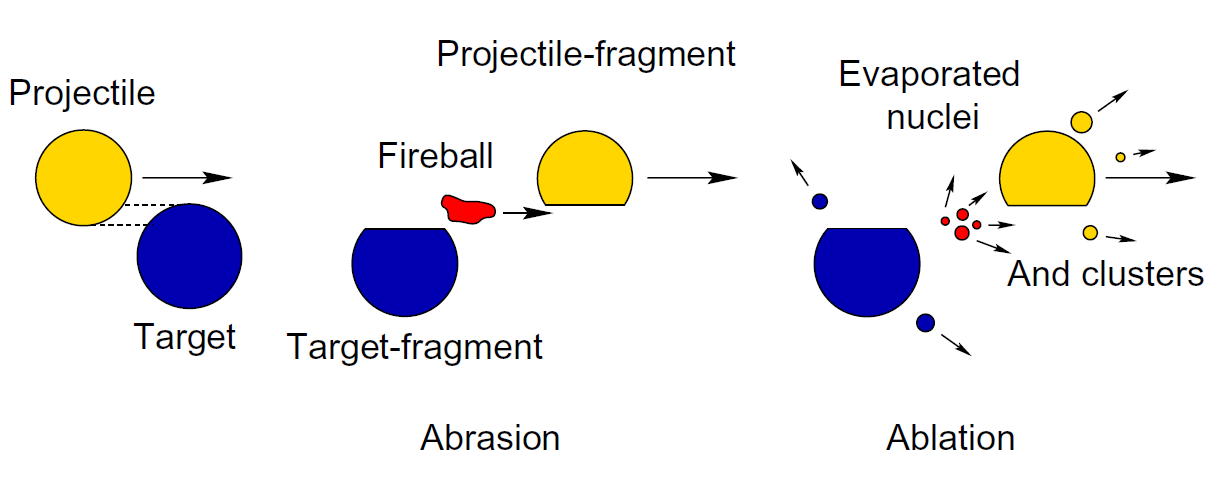
\includegraphics[width=0.5\textwidth]{images/ablationabration.png}  
\caption{Schematic of the physics involved.}
 \label{fig:ablationabration}
 \end{center}
 \end{figure}


\section{Simulation setup}
\begin{itemize}
\item Experiment data from GSI
\item target description
\item Characterization of the beam
\item Simulation of detectors
\item Implementation details
\end{itemize}

\section{Results and comparison to GSI data}
\begin{itemize}
\item comparison (Haettner 5.4.1)
\item energy distribution of fragments
\end{itemize}

\section{Conclusion}
\begin{itemize}
\item Raflaava yhteenveto
\end{itemize}

\section{Appendices}
\begin{itemize}
\item code examples
\item runtime log
\end{itemize}





\bibliographystyle{plain} \bibliography{refs.bib} 
\end{document}

\else

\fi